% Options for packages loaded elsewhere
\PassOptionsToPackage{unicode}{hyperref}
\PassOptionsToPackage{hyphens}{url}
%
\documentclass[
  9pt,
  ignorenonframetext,
]{beamer}
\usepackage{pgfpages}
\setbeamertemplate{caption}[numbered]
\setbeamertemplate{caption label separator}{: }
\setbeamercolor{caption name}{fg=normal text.fg}
\beamertemplatenavigationsymbolsempty
% Prevent slide breaks in the middle of a paragraph
\widowpenalties 1 10000
\raggedbottom
\setbeamertemplate{part page}{
  \centering
  \begin{beamercolorbox}[sep=16pt,center]{part title}
    \usebeamerfont{part title}\insertpart\par
  \end{beamercolorbox}
}
\setbeamertemplate{section page}{
  \centering
  \begin{beamercolorbox}[sep=12pt,center]{part title}
    \usebeamerfont{section title}\insertsection\par
  \end{beamercolorbox}
}
\setbeamertemplate{subsection page}{
  \centering
  \begin{beamercolorbox}[sep=8pt,center]{part title}
    \usebeamerfont{subsection title}\insertsubsection\par
  \end{beamercolorbox}
}
\AtBeginPart{
  \frame{\partpage}
}
\AtBeginSection{
  \ifbibliography
  \else
    \frame{\sectionpage}
  \fi
}
\AtBeginSubsection{
  \frame{\subsectionpage}
}
\usepackage{lmodern}
\usepackage{amsmath}
\usepackage{ifxetex,ifluatex}
\ifnum 0\ifxetex 1\fi\ifluatex 1\fi=0 % if pdftex
  \usepackage[T1]{fontenc}
  \usepackage[utf8]{inputenc}
  \usepackage{textcomp} % provide euro and other symbols
  \usepackage{amssymb}
\else % if luatex or xetex
  \usepackage{unicode-math}
  \defaultfontfeatures{Scale=MatchLowercase}
  \defaultfontfeatures[\rmfamily]{Ligatures=TeX,Scale=1}
\fi
\usetheme[]{Goettingen}
\usecolortheme{rose}
% Use upquote if available, for straight quotes in verbatim environments
\IfFileExists{upquote.sty}{\usepackage{upquote}}{}
\IfFileExists{microtype.sty}{% use microtype if available
  \usepackage[]{microtype}
  \UseMicrotypeSet[protrusion]{basicmath} % disable protrusion for tt fonts
}{}
\makeatletter
\@ifundefined{KOMAClassName}{% if non-KOMA class
  \IfFileExists{parskip.sty}{%
    \usepackage{parskip}
  }{% else
    \setlength{\parindent}{0pt}
    \setlength{\parskip}{6pt plus 2pt minus 1pt}}
}{% if KOMA class
  \KOMAoptions{parskip=half}}
\makeatother
\usepackage{xcolor}
\IfFileExists{xurl.sty}{\usepackage{xurl}}{} % add URL line breaks if available
\IfFileExists{bookmark.sty}{\usepackage{bookmark}}{\usepackage{hyperref}}
\hypersetup{
  pdftitle={BIOS6643 Longitudinal},
  pdfauthor={EJC},
  hidelinks,
  pdfcreator={LaTeX via pandoc}}
\urlstyle{same} % disable monospaced font for URLs
\newif\ifbibliography
\setlength{\emergencystretch}{3em} % prevent overfull lines
\providecommand{\tightlist}{%
  \setlength{\itemsep}{0pt}\setlength{\parskip}{0pt}}
\setcounter{secnumdepth}{-\maxdimen} % remove section numbering
\AtBeginSubsection{}
\AtBeginSection{}
\ifluatex
  \usepackage{selnolig}  % disable illegal ligatures
\fi

\title{BIOS6643 Longitudinal}
\subtitle{L4 LMM Foundation II: Random intercept model and RM ANOVA}
\author{EJC}
\date{}
\institute{Department of Biostatistics \& Informatics}

\begin{document}
\frame{\titlepage}

\begin{frame}[allowframebreaks]
  \tableofcontents[hideallsubsections]
\end{frame}
\hypertarget{background}{%
\section{Background}\label{background}}

\begin{frame}{Background}
\protect\hypertarget{background-1}{}
\begin{itemize}
\item
  One of the simplest ways to account for correlated data in a linear
  mixed model is to add a random intercept term. For example, adding a
  random intercept term for subjects will induce correlation between
  measures within subjects, even when repeated measures are not
  accounted for in the error covariance matrix.
\item
  The covariance structure (compound symmetric) is simplistic and often
  not realistic for longitudinal data (covariance between any pair of
  responses over time is the same regardless of the pair of time points
  being considered), but is far better than not accounting for
  correlation at all. When the random intercept term is for, say,
  schools, then the covariance structure might be more realistic.
\end{itemize}
\end{frame}

\begin{frame}{}
\protect\hypertarget{section}{}
\begin{itemize}
\item
  For the random-intercept-for subjects model we assume the random
  intercepts are drawn from a normal distribution with mean 0 and
  variance \(\sigma _b^2\) (i.e., between-subject variance).
\item
  When the error covariance matrix has the form \(\sigma_\epsilon^2I\),
  the model variance for a response at any time point is the sum of
  residual variance (or within-subject variance after accouting for
  fixed effects) and the between-subject variance.
\item
  The correlation between any 2 time points is the intraclass
  correlation coefficient
  \(\sigma _b^2 / (\sigma _b^2 + \sigma _\epsilon ^2)\). The analysis,
  or at least much of it, can be carried out using what is referred to
  Repeated Measures ANVOA (RM ANOVA), which has been around much longer
  than mixed models have, at least in practice. The model for the RM
  ANOVA can be considered as a special case of the LMM.
\end{itemize}
\end{frame}

\begin{frame}{Fitness data}
\protect\hypertarget{fitness-data}{}
\begin{itemize}
\item
  10 subjects were randomized to one of two fitness programs, one lower
  intensity and the other higher. Subjects were evaluated using an
  overall composite fitness score, which ranges from 0 to 75. Although
  it is an integer score, given the many possible levels, using a linear
  model has been shown to be adequate for the data. Subjects were
  evaluated at baseline (Week 0), and then at 4 successive weeks after
  starting the program (e.g., Week 1 as at the end of the first week),
  making for 5 times points per subject.
\item
  The fitness longitudinal data are shown below. Data suggests that the
  lower intensity program has bigger gains in early weeks, while the
  higher intensity program has stronger gains in later weeks. Data will
  be fit with a model to determine whether apparent differences are
  statistically significant.
\end{itemize}
\end{frame}

\begin{frame}{Fitness data figure}
\protect\hypertarget{fitness-data-figure}{}
\alert {need some figures}
\end{frame}

\begin{frame}{Understanding variation in the data}
\protect\hypertarget{understanding-variation-in-the-data}{}
\begin{itemize}
\item
  Analysis of variance (ANOVA) tables are intuitive, as they partition
  total (corrected) sums of squares into sources, providing a sense of
  relative amounts of variation in the data.
\item
  Repeated measures ANOVA (RM ANOVA) uses the standard ANOVA approach,
  but makes adjustments to tests to account for the repeated measures
  taken within subjects.
\item
  These days, linear mixed models can be used to achieve the same
  analysis, so there is no need to perform an RM ANOVA via PROC GLM. The
  RM ANOVA just helps give us an intuitive understanding for the sources
  of variation.
\item
  In general, inference in LMMs are not based on ANOVA tables, but in
  some cases like this one, inference is the same.
\end{itemize}
\end{frame}

\begin{frame}{}
\protect\hypertarget{section-1}{}
\begin{itemize}
\item
  In order to consider variation and the RM ANOVA approach, consider the
  following model.

  \(Y_{hij} = \mu \ + \gamma _{h(Group)} + \tau _{j(Time)} + (\gamma \tau )_{hj (Group \times Time)}\ + b_{i:h(Subject:Group)} + \epsilon _{hij(error)}\);\\
  where \(b_{i(h)} \stackrel {iid} \sim \mathcal N(0,\ \sigma _b^2)\)
  independent of
  \(\epsilon _{hij} \stackrel {iid} \sim \mathcal N(0,\  \sigma _\epsilon ^2)\).
\item
  Sum to \(0\) restrictions can be placed on \(G\), \(T\) and
  \(G \times T\) effects. Although the subject term is random, for RM
  ANOVA, subjects within groups is treated as a fixed-effect term, at
  least initially (i.e., within PROC GLM, and ID(PROGRAM) is added as a
  term in the MODEL statement). This allows us to incorporate all
  sources of variation in the table.
\end{itemize}
\end{frame}

\hypertarget{repeated-measures-anova}{%
\section{Repeated measures ANOVA}\label{repeated-measures-anova}}

\begin{frame}{Repeated measures ANOVA}
\protect\hypertarget{repeated-measures-anova-1}{}
The ANOVA table, including expected mean squares. Note: \(Q_T\) is a
function of time effects; the greater the value, the more the difference
between \(\tau_j\) parameters. Similar for \(G\), \(G \times T\). In the
table above, \(n_h\) = number of subjects in group \(h\),
\(n_{tot}=total\) sample size.

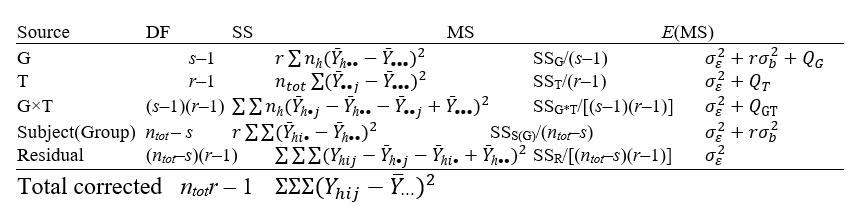
\includegraphics[width=1\linewidth]{figs_L4/f1}
\end{frame}

\begin{frame}{Tests (based on sum-to-0 restrictions)}
\protect\hypertarget{tests-based-on-sum-to-0-restrictions}{}
\begin{itemize}
\item
  \(Group \times Time\)

  \(H_0: \forall\ (\gamma \tau )_{hj} = 0 (or\ Q_{GT}=0)\)\\
  Use \(F = MS_{GT}/MS_{R}\)
\item
  Group

  \(H_0: \forall\ \gamma_h = 0 (or\ Q_G=0)\)\\
  Use \(F = MS_G/MS_{S(G)}\)
\item
  Subject (i.e., Subject(Group))\\
  \(H_0: \sigma_b^2 = 0\)\\
  Use \(F = MS_{S(G)}/MS_R\)
\item
  Time \(H_0: \forall\  \tau_j = 0 (or\ Q_T=0)\)\\
  Use \(F = MS_T/MS_R\)
\end{itemize}

\textbf{Estimating the ICC may be more informative than running a test
for subject variance.}
\end{frame}

\begin{frame}{ANOVA table}
\protect\hypertarget{anova-table}{}
The observed ANOVA table for our model is as follows.\\
Included here is another row for Model, which is the sum of all other
sources expect Residual.

\alert {need dataset}
\end{frame}

\begin{frame}{}
\protect\hypertarget{section-2}{}
\begin{itemize}
\item
  If you do not identify the repeated measures within subjects, the
  Program effect is much more significant than it should be (crossed
  out).
\item
  Essentially, the Program effect is a between-subject effect, so it
  makes sense that the denominator MS for the corresponding \(F\)
  statistic is based on the Subject(Program) source of variability; this
  \(F\) statistic is much smaller. The other model sources use the
  standard residual source (\(MS_{Residual}\)) in the denominator of
  \(F\).
\item
  Subject(Program) allows us to estimate subject variability not due to
  Program effects; using Subject instead of Subject(Program) would not
  allow us to tease out Program variability from Subject variability.
\end{itemize}
\end{frame}

\begin{frame}{}
\protect\hypertarget{section-3}{}
\begin{itemize}
\item
  In general, the correct form of \(F\) can be guided by examining the
  expected mean squares.
\item
  Under the null hypothesis of no effect for the source in question, the
  expected MS should be the same in the numerator and denominator. For
  example, for the \(Group \times Time\) test, the \(E[MS]\) is
  \(\sigma _\epsilon^2+Q_{GT}\). Under the null, \(Q_{GT}=0\), reducing
  the quantity to \(\sigma _\epsilon^2\). Thus, the standard
  \(MS_{Residual}\) is the correct one.
\item
  On the other hand, for group,
  \(E[MS]= \sigma _\epsilon^2+r\sigma _b^2+Q_G\). Under the null,
  \(Q_G=0\), reducing the quantity to
  \(\sigma _\epsilon^2+r\sigma _b^2\), which is
  \(E[MS_{Subject(group)}]\), showing that \(MS_{Subject(group)}\) is
  the correct denominator term.
\end{itemize}
\end{frame}

\begin{frame}{}
\protect\hypertarget{section-4}{}
To carry out the RM ANOVA using PROC GLM, the basic code is shown below.

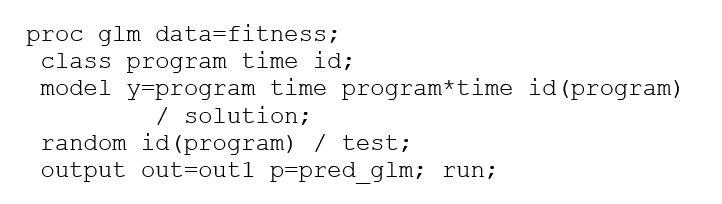
\includegraphics[width=1\linewidth]{figs_L4/f2}

\begin{itemize}
\item
  The total variability in the data, 8140.72, is the sum of squared
  distances from the overall mean to the data points. This is also often
  called `Corrected Total Sum of Squares', where the correction is for
  the mean.
\item
  The first partition of the data sums of squares is into portions
  attributed to Model and Error, 7441.44 and 699.28, respectively,
  demonstrating that the model can account for a large portion of
  variation in the data. Dividing these quantities by their respective
  degrees of freedom (17 and 32) yield Mean Square quantities of 437.7
  and 21.85, respectively.
\end{itemize}
\end{frame}

\begin{frame}{}
\protect\hypertarget{section-5}{}
\begin{itemize}
\item
  Method of moments can be used to obtain estimates of variance
  components in terms of Mean Square quantities. In particular,
  \(E[MS_{Subject(Group)}] = \sigma_\epsilon^2+r\sigma_b^2\) and
  \(E[MS_{Residual}] = \sigma_\epsilon^2\)
\item
  So we set the left side to MS quantities, put hats on variance terms
  on the right, and then solve for these estimated variance terms, to
  yield: \(\hat \sigma_\epsilon^2 = MS_{Residual}\) and
  \(\hat \sigma_b^2 = (MS_{Subject(Group)} - MS_{Residual})/r\)
\item
  For our data, these estimates are \(\hat \sigma_\epsilon^2=21.8525\)
  and \(\hat \sigma_b^2=(500.49 – 21.8525)/5 = 95.7525\).

  \begin{itemize}
  \tightlist
  \item
    These variances show that between-subject variability is about 5
    times larger than the within-subject variability that does not
    include variation due to the fixed effects.
  \end{itemize}
\item
  Two noticeable features in the data are the intercept variations in
  the `noodles' and the increase in noodles over time; these are the two
  greatest sources of variation in the mean-corrected SS:
  \(2788/8140 = 34%
  \) for Time and \(4004/8140 = 49%
  \) for subjects within programs, a total of \(83%
  \) of variation in the data.
\end{itemize}
\end{frame}

\hypertarget{the-lmm-approach}{%
\section{The LMM approach}\label{the-lmm-approach}}

\begin{frame}{The LMM approach}
\protect\hypertarget{the-lmm-approach-1}{}
\begin{itemize}
\item
  To fit the same model using an LMM, we treat subject as a true random
  effect (subject intercept here).
\item
  Similarities between RM ANOVA and LMM approaches:

  \begin{itemize}
  \item
    Using REML, the estimated variances are exactly the same as using
    method of moments with RM ANOVA.
  \item
    The estimates of fixed effects for Program, Time and
    \(Program \times Time\) effects are exactly the same.
  \end{itemize}
\end{itemize}
\end{frame}

\begin{frame}{}
\protect\hypertarget{section-6}{}
\begin{itemize}
\item
  Differences between approaches

  \begin{itemize}
  \item
    Subjects(Program) is treated as a fixed effect with the RM ANOVA
    approach, and random for the LMM approach. This leads to differences
    in subject-specific estimates.
  \item
    Specifically, since empirical Bayes methods are used to estimate
    random effects for subjects, the predicted values for subjects that
    incorporate random effect estimates will be shrunk back to the
    overall mean to some degree, relative to the GLM estimates that
    treat subject effect as fixed effects.
  \item
    This is demonstrated in the following graph; the LMM estimates are
    in solid blue and the GLM estimates are in dashed red. The
    differences in this case are not great, but clearly the LMM
    estimates are compressed to the middle relative to the GLM
    estimates. The more reliable subject data are (more values, less
    variability), the less the shrinkage. This probably explains the
    small amount of shrinkage here.
  \end{itemize}
\end{itemize}
\end{frame}

\begin{frame}{figures}
\protect\hypertarget{figures}{}
\alert {lmm blup figure}
\end{frame}

\begin{frame}{}
\protect\hypertarget{section-7}{}
\begin{itemize}
\item
  For any other differences between RM ANOVA and LMM, I would recommend
  using the latter, since subjects are modeled using random effects,
  i.e., they are considered as having been sampled from a normal
  population, and inference properly accounts for this.
\item
  If we are interested in inference just for the sample of subjects
  used, it makes sense to treat them as fixed effects, but usually we
  are more interested in the general population they were sampled from.
\item
  Differences in approaches is reflected in the lower standard errors of
  estimates in the RM ANOVA approach relative to the LMM approach. With
  RM ANOVA, Subjects-within-Programs is modeled as a fixed effect; hence
  inference is conditioned on the particular subjects at hand; for the
  LMM approach, inference for fixed effects is based on the marginal
  model (averaging over subjects in the population), naturally (and
  appropriately) leading to larger SE's.
\end{itemize}
\end{frame}

\begin{frame}{}
\protect\hypertarget{section-8}{}
\begin{itemize}
\item
  Basic SAS code to fit the model above is shown below. The OUTP will
  provide BLUP estimates for each value in the data set
  (\(\pmb {\hat Y=X \hat \beta + Zb}\)), while OUTPM provides
  \(\pmb {\hat Y= X \hat \beta}\).
\item
  The LSMEANS statement will provide estimates for each
  \(Program \times\) time combination. Adding the `diff' option to the
  right of the slash will provide comparisons between all pairs of
  differences in these combinations. There are also options to control
  for multiple testing using the Adjust option. For more detail, see the
  SAS Help Documentation.
\item
  The `solution' option in the RANDOM statement provides estimates and
  \(t\)-tests for random effect estimates (the same solution option
  could be added in the MODEL statement, but the LSMEANS options gives
  us what we need in this case).
\end{itemize}
\end{frame}

\begin{frame}{}
\protect\hypertarget{section-9}{}
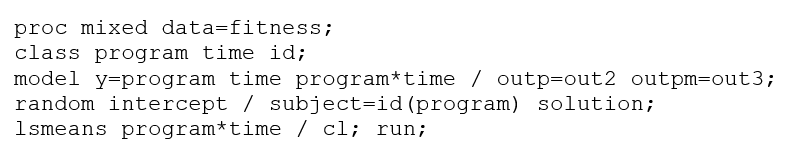
\includegraphics[width=1\linewidth]{figs_L4/f3}

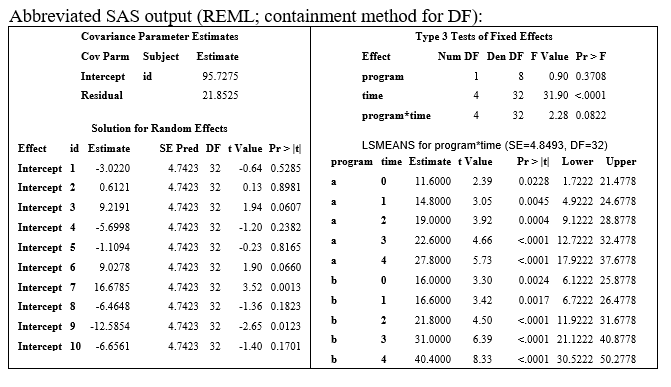
\includegraphics[width=1\linewidth]{figs_L4/f4}
\end{frame}

\begin{frame}{}
\protect\hypertarget{section-10}{}
\begin{itemize}
\item
  One methodological difference in fitting LMM's is that in order to
  conduct inference, we develop statistical quantities that have
  approximate t or F distributions, and then estimate the denominator
  degrees of freedom to conduct `correct' inference.
\item
  There are 6 or 7 different methods that can be used, and in SAS, the
  default methods used will depend on how the model is specified. This
  will be discussed more later, but for our purposes now, an important
  thing to realize is that SAS and R have different default methods,
  which is why results may appear slightly different.
\item
  For the SAS code above, the default denominator degrees of freedom
  (DDFM) method used is the `Containment', since there is a RANDOM
  statement. In order to change the method, you can add the DDFM option
  to the right of the slash in the MODEL statement.
\end{itemize}
\end{frame}

\begin{frame}{}
\protect\hypertarget{section-11}{}
\begin{itemize}
\tightlist
\item
  Basic R code using the \textbf{lme4::lmer()} function from the
  \textbf{lme4} package. Note that there are 3 basic DDFM methods
  available, two approximate (Satterthwaite, Kenward-Roger), and
  asymptotic. Asymptotic is not recommended for smaller data sets, as it
  is likely to lead to inflated Type I error rates and CI's that are too
  narrow.
\end{itemize}

\alert {need dataset}
\end{frame}

\begin{frame}{}
\protect\hypertarget{section-12}{}
Note that the results above match the RM ANOVA approach for the balanced
fitness data. The estimated marginal means (\textbf{emmeans()}) are the
same as the LSMEANS from SAS's approach. The only difference between SAS
and R in the analysis is in the CI's and p-values, which is due to
different DDFM methods used (Satterthwaite here, Containment using SAS).

Summary of DDF's for different DDFM methods for Fitness data, with the
Random intercept model

\alert {need dataset for table and figures}
\end{frame}

\hypertarget{summary}{%
\section{Summary}\label{summary}}

\begin{frame}{Summary}
\protect\hypertarget{summary-1}{}
\end{frame}

\end{document}
